%%%%%%%%%%%%%%%%%%%%%%%%%%%%%%%%%%%%%%%%%
% Journal Article
% LaTeX Template
% Version 1.4 (15/5/16)
%
% This template has been downloaded from:
% http://www.LaTeXTemplates.com
%
% Original author:
% Frits Wenneker (http://www.howtotex.com) with extensive modifications by
% Vel (vel@LaTeXTemplates.com)
%
% License:
% CC BY-NC-SA 3.0 (http://creativecommons.org/licenses/by-nc-sa/3.0/)
%
%%%%%%%%%%%%%%%%%%%%%%%%%%%%%%%%%%%%%%%%%

%----------------------------------------------------------------------------------------
%	PACKAGES AND OTHER DOCUMENT CONFIGURATIONS
%----------------------------------------------------------------------------------------

%\documentclass{article}
\documentclass[oneside,twocolumn]{article}

\usepackage{blindtext} % Package to generate dummy text throughout this template 
\usepackage{multicol}
\usepackage[sc]{mathpazo} % Use the Palatino font
\usepackage[T1]{fontenc} % Use 8-bit encoding that has 256 glyphs
\linespread{1.05} % Line spacing - Palatino needs more space between lines
\usepackage{microtype} % Slightly tweak font spacing for aesthetics

\usepackage[english]{babel} % Language hyphenation and typographical rules

\usepackage[hmarginratio=1:1,top=32mm,columnsep=20pt]{geometry} % Document margins
\usepackage[hang, small,labelfont=bf,up,textfont=it,up]{caption} % Custom captions under/above floats in tables or figures
\usepackage{booktabs} % Horizontal rules in tables

\usepackage{lettrine} % The lettrine is the first enlarged letter at the beginning of the text

\usepackage{enumitem} % Customized lists
\setlist[itemize]{noitemsep} % Make itemize lists more compact

\usepackage{abstract} % Allows abstract customization
\renewcommand{\abstractnamefont}{\normalfont\bfseries} % Set the "Abstract" text to bold
\renewcommand{\abstracttextfont}{\normalfont\small\itshape} % Set the abstract itself to small italic text

\usepackage{titlesec} % Allows customization of titles
\renewcommand\thesection{\Roman{section}} % Roman numerals for the sections
\renewcommand\thesubsection{\roman{subsection}} % roman numerals for subsections
\titleformat{\section}[block]{\large\scshape\centering}{\thesection.}{1em}{} % Change the look of the section titles
\titleformat{\subsection}[block]{\large}{\thesubsection.}{1em}{} % Change the look of the section titles

\usepackage{fancyhdr} % Headers and footers
\pagestyle{fancy} % All pages have headers and footers
\fancyhead{} % Blank out the default header
\fancyfoot{} % Blank out the default footer
%\fancyhead[C]{Running title $\bullet$ May 2016 $\bullet$ Vol. XXI, No. 1} % Custom header text
\fancyfoot[RO,LE]{\thepage} % Custom footer text

\usepackage{titling} % Customizing the title section

\usepackage{hyperref} % For hyperlinks in the PDF

\usepackage{listings}
\usepackage{algorithm2e}
\usepackage{graphicx}
\usepackage[dvipsnames]{xcolor}
\definecolor{codegreen}{rgb}{0,0.6,0}
\definecolor{codegray}{rgb}{0.5,0.5,0.5}
\definecolor{codepurple}{rgb}{0.58,0,0.82}
\definecolor{backcolour}{rgb}{1,1,1}
\lstdefinestyle{mystyle}{
    backgroundcolor=\color{backcolour},   
    commentstyle=\color{codegreen},
    keywordstyle=\color{magenta},
    numberstyle=\tiny\color{codegray},
    stringstyle=\color{codepurple},
    basicstyle=\ttfamily\footnotesize,
    breakatwhitespace=false,         
    breaklines=true,                 
    captionpos=b,                    
    keepspaces=true,                 
    numbers=left,                    
    numbersep=5pt,                  
    showspaces=false,                
    showstringspaces=false,
    showtabs=false,                  
    tabsize=2
}
\renewcommand{\lstlistingname}{Código}% Listing -> Algorithm
\lstset{style=mystyle}

%----------------------------------------------------------------------------------------
%	TITLE SECTION
%----------------------------------------------------------------------------------------

\setlength{\droptitle}{-4\baselineskip} % Move the title up

\pretitle{\begin{center}\Huge\bfseries} % Article title formatting
\posttitle{\end{center}} % Article title closing formatting
\title{Propagación de frente de onda} % Article title
\author{%
\textsc{Luis Alberto Ballado Aradias} \\%\thanks{A thank you or further information} \\[1ex] % Your name
\normalsize Cinvestav Unidad Tamaulipas \\ % Your institution
\normalsize luis.ballado@cinvestav.mx % Your email address
%\and % Uncomment if 2 authors are required, duplicate these 4 lines if more
%\textsc{Jane Smith}\thanks{Corresponding author} \\[1ex] % Second author's name
%\normalsize University of Utah \\ % Second author's institution
%\normalsize \href{mailto:jane@smith.com}{jane@smith.com} % Second author's email address
}
\date{\today} % Leave empty to omit a date
\renewcommand{\maketitlehookd}{%
\begin{abstract}
\noindent The task of building a map of an unknown environment and concurrently using that map to navigate is a central problem in mobile robotics research. This document trys to replicate one of the knows algorithm (wavefront expansion) to explore a map using C++ code in the first phase and parallelizate it to perform its calculations trying to reduce the total computation time. Parallel wavefront expansion can significantly improve the computational performance and speed of the algorithm, particularly when processing large environments or complex obstacles. By utilizing multiple processing units, the algorithm should process the environment, reducing the total computation time. However, parallel software also has some limitations, such as increased complexity in implementation and increased communication overhead between processing units. It is important to consider these limitations.

\end{abstract}
}

%----------------------------------------------------------------------------------------

%One of the major applications of mobile robots is to create models of the environment they traverse using sensor data; this process is known as mapping. Military applications of this technology are obvious. Visualize a robot that somehow enters a vacant building in hostile territory. For example, it could be thrown through an open window, crawl through drain pipes, or climb up the side of the building. Once inside, the robot can traverse the hallways and create a map showing doors, hall crossing, stairways, and other features.

%The most commonly used approaches to mapping are termed "grid based or metric mapping and topological mapping".
%Metric or quantitative maps, as the name implies, are based on measurements of the space they map. An indoor metric map may include the lengths of wall sections, door-opening widths, hallways widths, distances to intersections, and so forth. A typical metric navigation instruction might be "Move 45 meters in north direction, then turn 30º clockwise and move another 65 meters.
%Path planning in metrically mapped spaces usually includes the designation of a number of way points at specific (x,y) locations, connected by straight-line segments. Paths can then be selected on the basis of some optimization criterion.
%A widely used method of generationg a metric map is to cover the environment to be mapped with an evently spaced grid. Each cell in the grid is then filled with one or more values that represent the presence or absence of an obstacle (which could be another robot or a human).Grid-based mapping was first proposed in the 1980's  by Elfes

\begin{document}

% Print the title
\maketitle

%----------------------------------------------------------------------------------------
%	ARTICLE CONTENTS
%----------------------------------------------------------------------------------------


    
\section{Introducción}

\lettrine[nindent=0em,lines=3]{L} a propagación del frente de onda es un algoritmo popular para la planificación de rutas en robótica móvil, es usado para determinar el camino óptimo para que un robot se mueva desde su punto de inicio a un objetivo en particular. Evitando obstáculos que pueda presentar a su paso. El algoritmo comienza con la posición destino y crea movimientos de exploración en sus vecindarios creando un frente de onda que se expande (como una onda alrededor), se debe actualizar el costo de navegar a cada nueva casilla. La ruta final es determinada seleccionando el gradiente de menor costo hasta la posición final establecida.\\

Desde la epoca de los 60s, la planificación de rutas a tenido un gran interés. La planificación de rutas es un problema que se puede describir de la siguiente manera: dado un robot que conoce su entorno, el robot móvil buscará un camino óptimo o sub-óptimo desde su posición inicial hacia el objetivo marcado acorde al criterio del entorno en el que navega. El uso de buenos planificadores aplicados a la robótica móvil puede no solo ayudar mucho tiempo en su desplazamiento, si no también reducir algunos recursos vitales en la robótica como lo es el consumo de energía.\\

La propagación de frente de onda es de gran ayuda cuando a priori se conoce el mapa del robot, y puede ser usado a su beneficio eficientando su tiempo de computo en aplicaciones en tiempo real. El algoritmo puede soportar ambientes simples como complejos, con muchos y pocos obstáculos produciendo una ruta óptima, conociendo si existe o no un camino en un tiempo relativamente corto. Adicional a ello, podemos dotar al algoritmo de mayor complejidad incorporando funciones de costo por desplazamiento de punto A $\rightarrow$ B en cuestiones de energía añadiendo diferentes consideraciones a su función de costo por visitar una nueva celda.\\

Uno de los beneficios de la propagación del frente de onda es su simplicidad, que la hace fácil de entender e implementar en lenguajes como C++ haciendo uso de estructuras como Queues (Colas). El algoritmo parte de su similitud al algoritmo de búsqueda en anchura (BFS), es por eso que se optó en cambiar la implementación para hacer uso de la representación del mapa en una estructura tipo grafo haciendo más entendible, pero a mi persona complicada la implementación. Pero una vez entendiendo la sintaxis del lenguaje C++ y el uso correcto de estructuras y la representación del mapa como una lista de adyacencia fué posible hacer uso del algoritmo en su forma correcta.\\

Aunque, la propagación del frente de onda tiene sus limitaciones, es caso de estudio para llegar a una eficiente implementación en una versión paralela.\\

\textbf{Búsqueda en anchura (BFS - Breadth First Search)}, desde la universidad me facinaba y sorprendian los videos asiaticos de concursos de robótica, en donde resuelven un laberinto en cuestion de segundos \href{https://www.youtube.com/watch?v=kMOssi5IcP0}{ver video}, en ese momento sabia que lo resolvian mapeando antes el entorno y por las clases de matemáticas discretas lo resolvian aplicando algún algoritmo para grafos, pero desconocia del tema, al tomar la clase de Análisis y Diseño de Algoritmos y tomar algunas sesiones de algoritmos para grafos quede fascinado de su aplicación en el mundo real fuera de los tipicos ejemplos de redes sociales, ahí comprendí que es un campo ahora de mi interés replantiandome de nuevo el problema y viendolo como un grafo. Aplicando el algoritmo BFS cuya particularidad es encontrar el camino más corto en un grafo ponderado, el algoritmo inicia en algún nodo del grafo y explora los nodos vecinos primero antes de moverse al siguiente nodo.\\

Muchos problemas en teoria de grafos pueden ser representados usando matrices. Estos son grafos implicitos que podemos determinar los vecinos del nodos basados en la ubicación en la matriz.\\

Una forma de resolver problemas que pueden ser representados como matrices o gradillas, es primero convertir la matriz a un formato como una lista de adyacencia, esta lista representará los vecinos de dicho nodo. Partiendo que en nuestro problema se pueden presentar obstáculos que pueden incomunicar el camino de un nodo a otro que en nuestro caso es representado por \# , cada que encontremos dicho simbolo será omitido de ser agregado a la representación de su lista de adyacencia.\\

\textbf{Dirección de exploración} Dado a que la estructura inicial es una gradilla, sabemos que nos podemos mover hacia direcciones como izquierda, derecha, arriba y abajo. Matemáticamente si partimos de una posición conocida (fila,columna), podemos hacer desplazamientos de fila-1,columna; fila,columna+1, fila+1,columna o fila,columna-1 para alcanzar las celdas adyacentes. Esto hace muy sencillo el acceso a los nodos vecinos desde un nodo dado.\\

Hay una necesidad creciente en la exploración y análisis de grafos a gran escala en computación, redes sociales, y análisis de negocios. Aunque por la irregularidad e intenso uso de memoria, las aplicaciones en grafos son conocidos por su ineficiente y pobre performance en computación paralela haciendo un reto la paralelización de un algoritmo como BFS, encontrandose con cuellos de botella que aunque existen métodos que dan solución logrando separarlos en multiples hilos, en el presente trabajo no llegamos a explorarlos. Haciendo una paralelización a nivel de problemas de agentes de robots. Es decir correr el algoritmo en paralelo en diferentes hilos y no paralelizando el algoritmo per sé.


%------------------------------------------------

\newpage
\onecolumn
\section{Algoritmo Secuencial}

La implementación tipica de la expansión del frente de onda, se parte de una representación de la matriz de entrada como una lista de adyacencia que representa un grafo, ordenando la lista de adyacencia por nodos y poder encolar los nodos para poder análisar y recorrer el grafo con ayuda de algoritmos como BFS.\\

El programa secuencial consiste en la invocación de las siguientes funciones:

\begin{itemize}
\item \textbf{main:} Dentro la función main, se hace la lectura del mapa, creando su representación matricial dentro del programa, para despues pasarlo a una representación de lista de adyacencia.
\item \textbf{bfs:} función principal del programa donde se desarrolla el algoritmo iterando respecto al número de robots a analizar
\item \textbf{get\_neighbors:} función para explorar los vecinos respecto a la matriz
\item \textbf{get\_workload:} función para dividir el trabajo respecto al numero de hilos y robots a repartir entre ellos
\item \textbf{print\_dist:} función que imprime y muestra la animación del frente de onda en la consola en tiempo real
\end{itemize}

Se crearon diversas banderas para la ejecución del programa en la terminal:

\begin{itemize}
\item -{}-MODE : las posibles opciones son SECUENCIAL y PTHREADS, forma de uso --MODE=SECUENCIAL ó --MODE=PTHREADS
\item -{}-SHOW : mostrar ó no la animación, forma de uso --SHOW
\item -{}-nth  : número de hilos (threads) a utilizar, forma de uso --nth=2
\item -{}-results : mostrar los resultados de los costos de visita a cada nodo del grafo
\item -{}-locations : archivo de la ubicación de los robots a ser analizados
\item -{}-robots : número de robots a ser analizados, la cardinalidad del archivo de locations debe considir con el número de robots, de lo contrario se presentará algún error de memoria por no ser iguales.  
\end{itemize}

Forma de correr el programa: \\

 \$ ./bfs < problem\_size/1M.txt -{}-MODE=PTHREADS -{}-robots=10 -{}-nth=2 -{}-locations=robots.txt -{}-results 

\subsection{main()}

En la función princial del programa, aunque mi forma de programar no fué la más sencilla y modular, dentro de esta parte se realizan las siguientes tareas:

\begin{itemize}
\item Definir las estructuras de datos a utilizar
\item Lectura de los argumentos de entrada (Banderas), respecto al MODO se corre la versión de PTHREADS o SECUENCIAL
\item Lectura del archivo de las ubicaciones de los robots, que será almacenado dentro de un vector de ubicaciones para ser accesado dentro del programa
\item Lectura la matriz (nuestro mapa) filas, columnas. Para así construir una matriz que podremos transformar a su representación de lista de adyacencia. \textbf{Se hace esete paso considerando el costo computacional del orden cuadratico, debido a que si en un primer barrido creo la lista de adyacencia y como condicion es saltarme el signo \# queda incompleta la representación del grafo, es por eso que primero construimos una matriz enbase de la lectura de la representación del mapa, para despues recorrerlo nuevamente aplicandole la exploracion de vecinos e ir agregando los nodos vecinos a su lista de adyacencia}
\item Mostrar resultados, si la bandera fué indicada proveniente de los argumentos de la terminal
\end{itemize}

\subsection{Frente de onda (BFS)}

\SetKwComment{Comment}{/* }{ */}

\begin{algorithm}
\caption{BFS}\label{alg:two}
$QUEUE \gets nodo\_inicio$ \Comment*[r]{Agregar nodo inicio a la cola}
$nodo\_inicio \gets visitado$ \Comment*[r]{Marcar el nodo inicio como visitado con costo 0}
agregar nodo a vector distancia $\gets 0$

\While{$!QUEUE.empty()$}{ \Comment*[r]{Hacer hasta no tener vecinos o nodos a explorar}
  $v \gets$ sacar nodo de QUEUE\;
  \For{para cada nodo adyacente del nodo dentro de $adj\_list[nodo]$}{
    \If{$nodo\_adj$ no ha sido visitado}{
      $QUEUE \gets nodo\_adj$ \Comment*[r]{Agregar nodo adyacente a la cola}
      $nodo\_adj \gets visitado$\; \Comment*[r]{Marcar el nodo como visitado con costo previo más uno}
      agregar a vector de distancia con costo $distancia[nodo]+1$\;
    }
  }
}
\end{algorithm}

La complejidad del algoritmo depende del tamaño del grafo, quedando directamente proporcional al número de vértices y aristas que éste contenga. En nuestro caso al no considerar una parada al encontrar el objetivo nuestro costo computacional es $O(|V|+|E|)$ ya que visita todos los vértices del grafo, donde V es el número de vértices y E es el número de aristas del grafo.\\

Como espacio computacional, al utilizar una estructura de datos tipo cola (queue) para guardar los nosdos que deben ser visitados, en nuestro caso debe visitar todos los nodos, haciendo la complejidad espacial a $O(V)$, donde V es el núm de nodos en el grafo. Por lo tanto la complejidad de nuestra implementación es $O(|V|+|E|)$ y en espacio $O(V)$ ya que no consideramos una condición de paro.

\newpage
\onecolumn
\section{Algoritmo Paralelo}

El Algoritmo de frente de onda es un algoritmo muy paralelizable repartiendo la carga de trabajo en la exploración de nuevos nodos dentro de la lista de adyacencia, dado que hacemos uso de una cola (queue) y para que el algoritmo siga funcionando todos los hilos deberán de agregar los nuevos nodos descubiertos a la misma cola compartida, es aquí donde se crea un cuello de botella. Conviertiendo nuestro algoritmo paralelo a secuencial nuevamente. Existen diversar formas de de evitarlo que no alcancé a explorar, algunas ideas es hacer uso de metodologias como work-stealing, donde cada hilo mantiene su propia cola, pero el hilo puede robar nodos de otros hilos cuando su cola este vacia. Creo que de esta forma se puede alcanzar un buen balanceo y escalabilidad buscada en un algoritmo paralelo, pero tiene un alto costo de sincronización.\\

En nuestro trabajo solamente exploramos el paralelizar la carga respecto a un número de robots a explorar, convirtiendo nuestro problema de partir el mapa a explorar a partir el trabajo en diferentes hilos para los diferentes robots que parten de diferentes ubicaciones.\\

Ahora el problema parte en repartir el trabajo respecto al número de hilos disponibles, es decir indicar a cada hilo cuantos robots le tocaron (función \textbf{get\_workload}) y que robots le tocaron pasandole un vector de las ubicaciones de robots indexado por el número de hilos indicado por el programa desde la ejecución de la terminal.\\

Como consideramos un vector de resultados para almacenar el costo por nodo desde su nodo inicio visitando cada uno de los nodos, es aquí donde presentamos una zona critica. Que es protegida con un mutex. Agradezco al Dr. Mario Garza-Fabre en ver mi error en su versión de OpenMP, ya que se presentaba un error que en mis experimentos y desarrollo nunca se me presento hasta la hora de correr los experimentos.

\newpage
\onecolumn
\section{Resultados}

Para la corrida del proyecto se creo una matriz de 1000 filas x 1000 columnas generada de manera aleatoria de forma artesanal, generando así 1 Millón de nodos de manera tal de estresar el algoritmo para ver tiempos grandes de ejecución. Para tamaños pequeños la animación -{}-SHOW está disponible teniendo un resultado como la siguiente imágen.\\

Para nuestros experimentos se proponen 5 tamaños de problemas que son el número de robots a analizar. \textbf{32, 64, 128, 256, 512}\\

\begin{figure}[h]
    \centering
    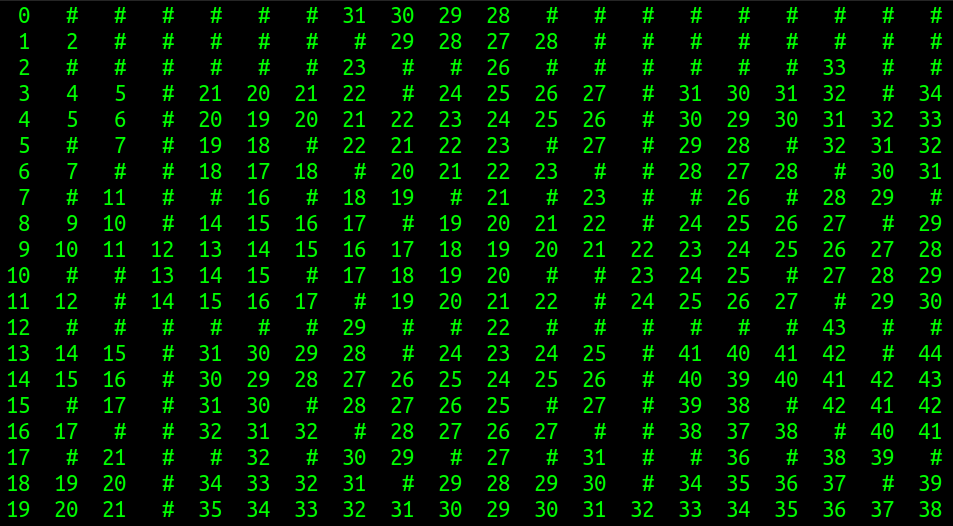
\includegraphics[width=0.80\textwidth]{grid.png}
    \caption{Grid de resultados}
    \label{fig:grid_resultados}
\end{figure}

\newpage
\subsection{Resultados Secuencial}

\begin{figure}[h]
    \centering
    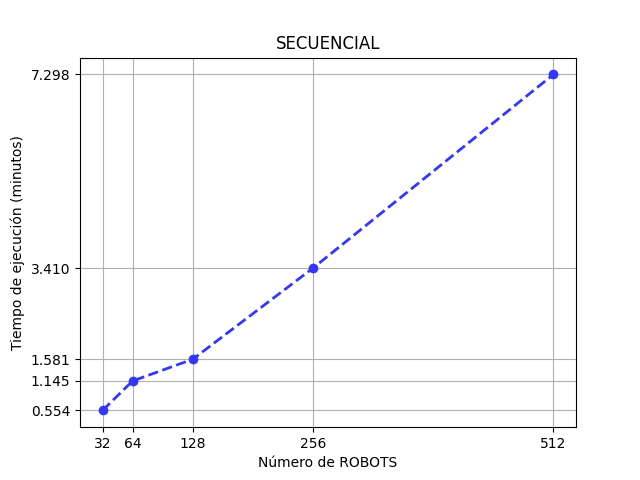
\includegraphics[width=0.80\textwidth]{graficos/secuencial/secuencial.png}
    \caption{Secuencial}
    \label{fig:secuencial}
\end{figure}

La tabla de resultados nos deja claro que a medida que incrementamos el número de robots que deben de explorar su nodo inicio con su nodo fin, el tiempo incrementa de forma casi lineal. Siendo un gran ejemplo de paralelización para observar los resultados, teniendo una gran similaridad con la complejidad de nuestro algoritmo $O(|V|+|E|)$

%TABLA SECUENCIAL
\begin{center}
\begin{tabular}{ |p{2cm}||p{4cm}| }
 \hline
 \multicolumn{2}{|c|}{SECUENCIAL} \\
 \hline
 ROBOTS & Tiempo (en minutos)\\
 \hline
 1    & 0.088\\
 \hline
 32   & 0.554\\ \hline
 64   & 1.024\\ \hline
 128  & 1.969\\ \hline
 256  & 3.683\\ \hline
 512  & 7.498\\ \hline
 \hline
\end{tabular}
\end{center}

\newpage
\onecolumn
\section{Resultados Pthreads}

Al paralelizar con la biblioteca Pthreads obtenemos grandes resultados en especial en nuestro problema que consta de 512 ROBOTS a analizar logrando bajar su tiempo de poco más de 7 Minutos en su corrida con 1 Hilo que tiene gran similaridad al tiempo obtenido en su versión secuencial a poquito mas de 1 Minuto haciendo uso de 32 Cores de la infraestructura del Cinvestav Unidad Tamaulipas. Es aquí donde se puede observar los beneficios y la importancia del uso de bibliotecas que nos permiten sacar el máximo de jugo a nuestros programas obteniendo grandes resultados.\\

El uso de pthreads nos permite mejorar la eficiencia, así como el rendimiento de nuestra aplicación haciendo que los hilos realicen varias tareas simultáneamente, reduciendo así el tiempo de ejecución, aumentando la velociadad de procesamiento. Pero como el antiguo adagio \textbf{Un gran poder conlleva una gran responsabilidad}.

\begin{figure}[h]
    \centering
    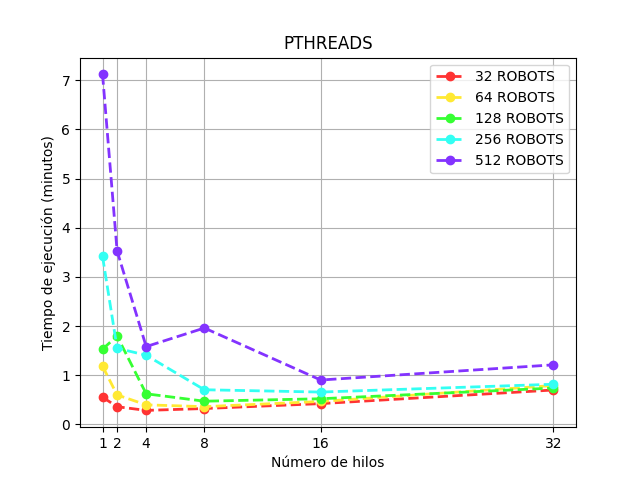
\includegraphics[width=0.80\textwidth]{graficos/pthreads/pthreads.png}
    \caption{Pthreads}
    \label{fig:secuencial}
\end{figure}

%TABLA PTHREADS
\begin{center}
\begin{tabular}{ |p{2cm}||p{2cm}||p{2cm}||p{2cm}||p{2cm}||p{2cm}||p{2cm}| }
 \hline
 \multicolumn{7}{|c|}{PTHREADS (tiempo en minutos)} \\
 \hline
 ROBOTS & 1 CORE & 2 CORE & 4 CORE & 8 CORE & 16 CORE & 32 CORE\\
 \hline
 32   & 0.554 & 0.359 & 0.284 & 0.322 & 0.422 & 0.699\\ \hline
 64   & 1.183 & 0.599 & 0.397 & 0.360 & 0.466 & 0.790\\ \hline
 128  & 1.530 & 1.796 & 0.622 & 0.471 & 0.521 & 0.739\\ \hline
 256  & 3.415 & 1.549 & 1.406 & 0.704 & 0.657 & 0.816\\ \hline
 512  & 7.119 & 3.527 & 1.582 & 1.960 & 0.902 & 1.211\\ \hline
 \hline
\end{tabular}
\end{center}

\newpage
\subsection{ACELERACION}

La aceleración usando pthreads nos proporciona una mejora muy significativa en el rendimiento de nuestro programa realizando multiples tareas simultáneamente. Al dividir la tarea que puede ser procesada en paralelo, se pueden aprovechar recursos de los múltiples núcleos de nuestra infraestructura disponible.\\

En nuestra imágen podemos observar la rápida aceleración a medida que va incrementando el problema llegando a su punto más alto, para después reducir su aceleración debido a que los hilos requieren cierta cantidad de recursos como memoria y procesamiento, a medida que aumentamos el número de cores, también se incrementa la latencia de la comunicación entre los hilos reduciendo la eficiencia, es por ello que se puede notar la reducción a medida que llegamos al número de cores que cuenta nuestro equipo.

\begin{figure}[h]
    \centering
    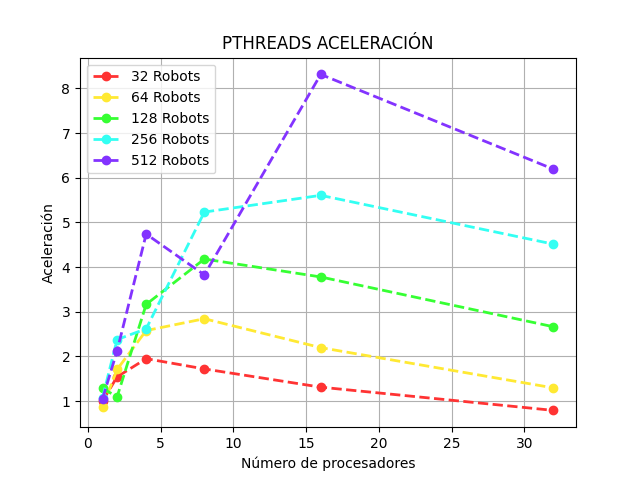
\includegraphics[width=0.80\textwidth]{graficos/pthreads/pth_acc.png}
    \caption{Pthreads Aceleración}
    \label{fig:secuencial}
\end{figure}

%TABLA PTHREADS ACELERACION
\begin{center}
\begin{tabular}{ |p{2cm}||p{2cm}||p{2cm}||p{2cm}||p{2cm}||p{2cm}||p{2cm}| }
 \hline
 \multicolumn{7}{|c|}{PTHREADS ACELERACION} \\
 \hline
 ROBOTS & 1 CORE & 2 CORE & 4 CORE & 8 CORE & 16 CORE & 32 CORE\\
 \hline
 32   & 1     & 1.543 & 1.950 & 1.720 & 1.312 & 0.796\\ \hline
 64   & 0.865 & 1.709 & 2.579 & 2.844 & 2.197 & 1.296\\ \hline
 128  & 1.286 & 1.096 & 3.165 & 4.180 & 3.779 & 2.664\\ \hline
 256  & 0.927 & 2.377 & 2.619 & 5.231 & 5.605 & 4.513\\ \hline
 512  & 1.053 & 2.125 & 4.739 & 3.825 & 8.312 & 6.191\\ \hline
 \hline
\end{tabular}
\end{center}

\newpage
\subsection{EFICIENCIA}

Podemos notar que nuestra eficiencia puede disminuir viendose afectada por diversas razones, como el tamaño del problema a resolver ó la implementación ineficiente de mis códigos o los problemas de comunicación entre los hilos. Como nuestro problema siempre lo estamos incrementando, cada vez requeire más memoria y tiempo de procesamiento para cada robot a analizar haciendo que la sobrecarga de recursos reduzca la eficiencia.

\begin{figure}[h]
    \centering
    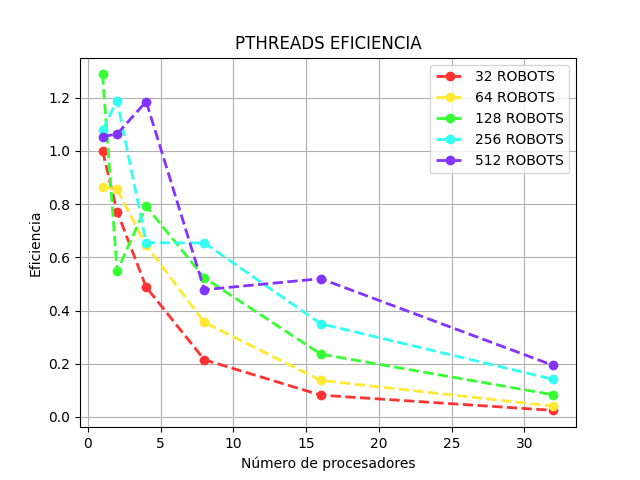
\includegraphics[width=0.80\textwidth]{graficos/pthreads/pthreads_eff.png}
    \caption{Pthreads Eficiencia}
    \label{fig:secuencial}
\end{figure}

%TABLA PTHREADS EFICIENCIA
\begin{center}
\begin{tabular}{ |p{2cm}||p{2cm}||p{2cm}||p{2cm}||p{2cm}||p{2cm}||p{2cm}| }
 \hline
 \multicolumn{7}{|c|}{PTHREADS EFICIENCIA} \\
 \hline
 ROBOTS & 1 CORE & 2 CORE & 4 CORE & 8 CORE & 16 CORE & 32 CORE\\
 \hline
 32   & 1     & 0.771 & 0.487 & 0.215 & 0.082 & 0.024\\ \hline
 64   & 0.865 & 0.854 & 0.644 & 0.355 & 0.137 & 0.040\\ \hline
 128  & 1.286 & 0.548 & 0.791 & 0.522 & 0.236 & 0.083\\ \hline
 256  & 0.927 & 1.188 & 0.654 & 0.653 & 0.350 & 0.141\\ \hline
 512  & 1.053 & 1.062 & 1.184 & 0.478 & 0.519 & 0.193\\ \hline
 \hline
\end{tabular}
\end{center}


\newpage
\onecolumn
\section{Resultados OpenMP}

Podemos observar la misma tendencia de resultados que con la biblioteca de Pthreads, no obstante la implementación de OpenMP fué más sencilla. Pero al no ser de grano fino, se presentaron condiciones de carrera que se puedieron observar en el servidor polifemo, teniendo una memoria corrupta. Gracias a la observación del Dr. Mario Garza-Fabre que logramos identificar y corregir la región critica en la escritura de un vector de resultados.

\begin{figure}[h]
    \centering
    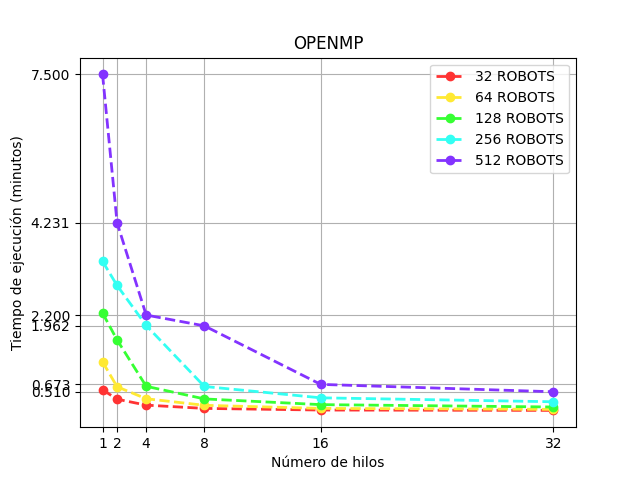
\includegraphics[width=0.80\textwidth]{graficos/openmp/openmp.png}
    \caption{OpenMP}
    \label{fig:secuencial}
\end{figure}

%TABLA OPENMP
\begin{center}
\begin{tabular}{ |p{2cm}||p{2cm}||p{2cm}||p{2cm}||p{2cm}||p{2cm}||p{2cm}| }
 \hline
 \multicolumn{7}{|c|}{OPEN MP (tiempo en minutos)} \\
 \hline
 ROBOTS & 1 CORE & 2 CORE & 4 CORE & 8 CORE & 16 CORE & 32 CORE\\
 \hline
 32   & 0.554 & 0.347 & 0.216 & 0.144 & 0.108 & 0.100\\ \hline
 64   & 1.170 & 0.621 & 0.357 & 0.212 & 0.144 & 0.123\\ \hline
 128  & 2.244 & 1.652 & 0.631 & 0.353 & 0.227 & 0.175\\ \hline
 256  & 3.383 & 2.851 & 1.971 & 0.627 & 0.377 & 0.290\\ \hline
 512  & 7.500 & 4.231 & 2.200 & 1.962 & 0.673 & 0.510\\ \hline
 \hline
\end{tabular}
\end{center}

\newpage
\subsection{ACELERACION}

\begin{figure}[h]
    \centering
    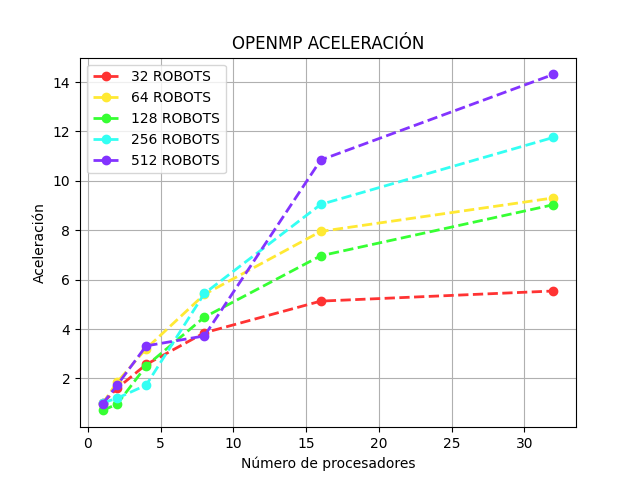
\includegraphics[width=0.80\textwidth]{graficos/openmp/openmp_acc.png}
    \caption{OpenMP Aceleración}
    \label{fig:secuencial}
\end{figure}

%TABLA OPENMP ACELERACION
\begin{center}
\begin{tabular}{ |p{2cm}||p{2cm}||p{2cm}||p{2cm}||p{2cm}||p{2cm}||p{2cm}| }
 \hline
 \multicolumn{7}{|c|}{OPEN MP ACELERACION} \\
 \hline
 ROBOTS & 1 CORE & 2 CORE & 4 CORE & 8 CORE & 16 CORE & 32 CORE\\
 \hline
 32   & 1     & 1.596 & 2.564 & 3.847 & 5.129  & 5.540\\ \hline
 64   & 0.875 & 1.648 & 2.868 & 4.830 & 7.111  & 8.325\\ \hline
 128  & 0.877 & 1.191 & 3.120 & 5.577 & 8.674  & 11.25\\ \hline
 256  & 1.088 & 1.291 & 1.868 & 1.868 & 9.769  & 12.70\\ \hline
 512  & 0.999 & 1.772 & 3.408 & 3.408 & 11.141 & 14.70\\ \hline
 \hline
\end{tabular}
\end{center}

\newpage
\subsection{EFICIENCIA}

\begin{figure}[h]
    \centering
    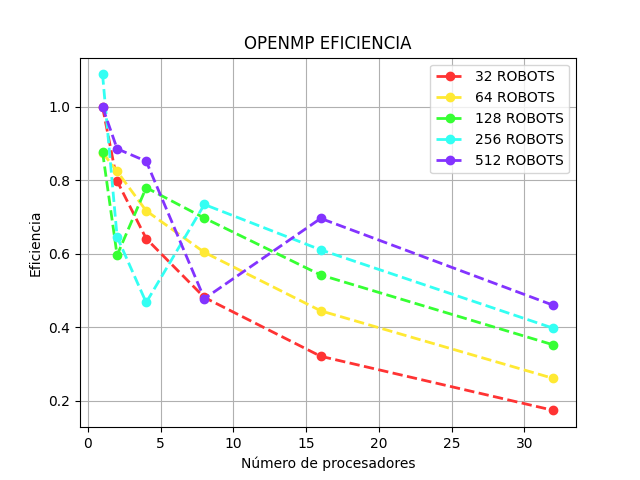
\includegraphics[width=0.80\textwidth]{graficos/openmp/openmp_eff.png}
    \caption{OpenMP Eficiencia}
    \label{fig:secuencial}
\end{figure}

%TABLA OPENMP EFICIENCIA
\begin{center}
\begin{tabular}{ |p{2cm}||p{2cm}||p{2cm}||p{2cm}||p{2cm}||p{2cm}||p{2cm}| }
 \hline
 \multicolumn{7}{|c|}{OPEN MP EFICIENCIA} \\
 \hline
 ROBOTS & 1 CORE & 2 CORE & 4 CORE & 8 CORE & 16 CORE & 32 CORE\\
 \hline
 32   & 1     & 0.798 & 0.641 & 0.480 & 0.320 & 0.173\\ \hline
 64   & 0.875 & 0.824 & 0.717 & 0.603 & 0.444 & 0.260\\ \hline
 128  & 0.877 & 0.595 & 0.780 & 0.697 & 0.542 & 0.351\\ \hline
 256  & 1.088 & 0.645 & 0.467 & 0.233 & 0.610 & 0.396\\ \hline
 512  & 0.999 & 0.886 & 0.852 & 0.426 & 0.696 & 0.459\\ \hline
 \hline
\end{tabular}
\end{center}

\newpage
\onecolumn
\section{Resultados Pthreads vs. OpenMP}

Ambas herramientas nos permiten paralelizar de forma eficiente atravez de múltiples cores de procesamiento. Teniendo mayor facilidad la biblioteca OpenMP en su implementación, pero siendo Pthreads la que nos ofrece mayor flexibilidad en terminos de como dividir la carga de trabajo en los hilos siendo este el grano fino de personalización que le da el toque que a mi gusto es más beneficioso.\\

Ambas bibliotecas pueden mejorar la eficiencia al distribuir la carga en los diferentes cores. Pero el rendimiento depende de la forma de su implementación.

\subsection{ACELERACION}

\begin{figure}[h]
    \centering
    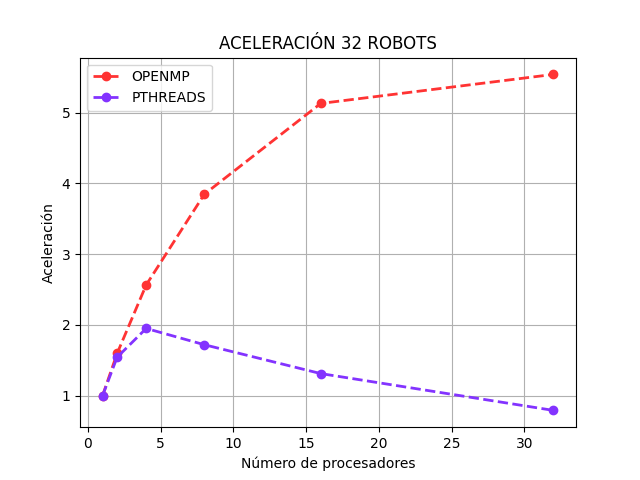
\includegraphics[width=0.80\textwidth]{graficos/comparacion/aceleracion_32.png}
    \caption{Aceleración 32 Robots}
    \label{fig:secuencial}
\end{figure}

\begin{figure}[h]
    \centering
    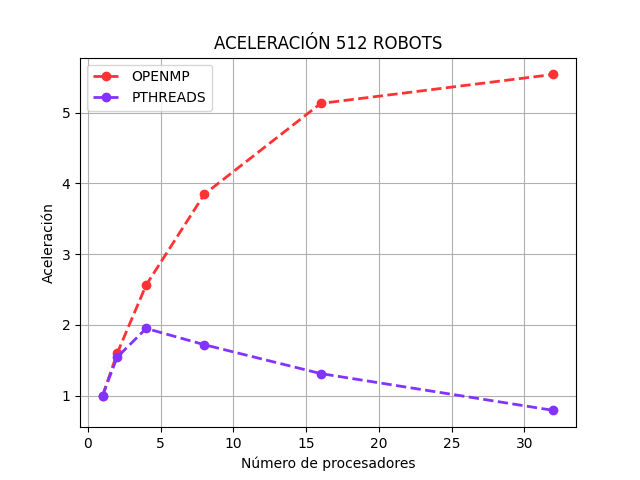
\includegraphics[width=0.80\textwidth]{graficos/comparacion/aceleracion_512.png}
    \caption{Aceleración 512 Robots}
    \label{fig:secuencial}
\end{figure}

\newpage
\subsection{EFICIENCIA}

\begin{figure}[h]
    \centering
    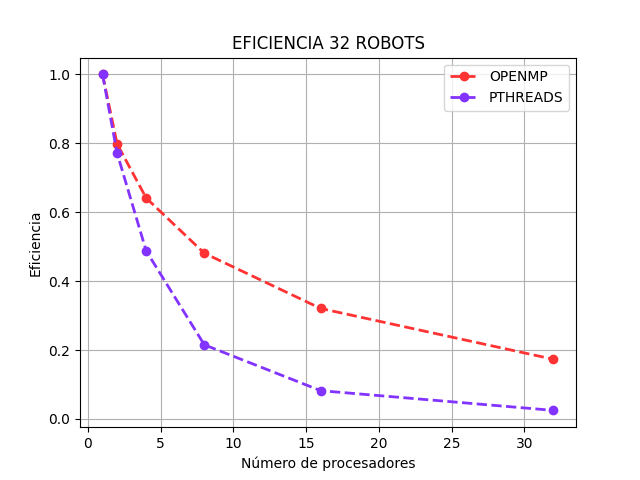
\includegraphics[width=0.80\textwidth]{graficos/comparacion/eficiencia_32.png}
    \caption{Eficiencia 32 Robots}
    \label{fig:secuencial}
\end{figure}

\begin{figure}[h]
    \centering
    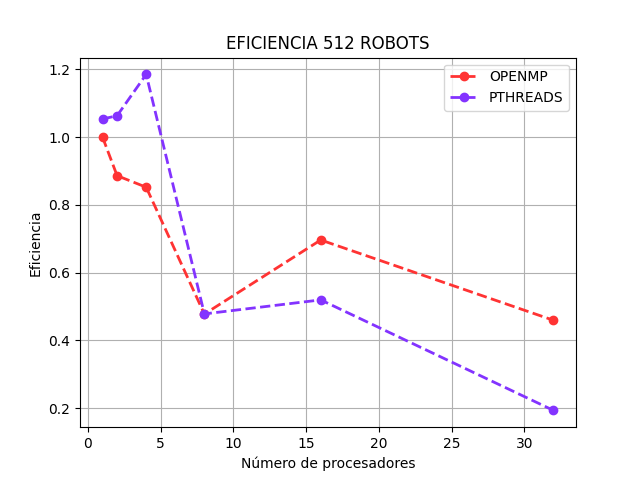
\includegraphics[width=0.80\textwidth]{graficos/comparacion/eficiencia_512.png}
    \caption{Eficiencia 512 Robots}
    \label{fig:secuencial}
\end{figure}

%------------------------------------------------

\newpage
\onecolumn
\section{Conclusions}

El algoritmo de propagación de frente de onda es una forma de procesar un grafo trabajando con vertices de forma de onda, donde los vertices en la misma onda pueden ser procesados de forma paralela con diversas técnicas que no logramos explorar en el prensente trabajo. El algoritmo al tener una base en BFS hizo que cambiaramos el plantamiento de nuestro problema.\\

El algoritmo de frente de onda sin la estructura de tipo Queue no resulta ser eficiente y me llego a ser confunsa por el barrido constante para poder alterar las distancias.\\

La programación paralela llevando un riguroso análisis se pueden obtener grandes beneficios, pero como dicta la ley de Amdahl que la parte secuencial de nuestro problema limita el rendimiento máximo que se puede obtener mediante la programación paralela, viendo el caso en que nuestro cuello de botella es la Cola donde almacenamos los siguientes nodos a visitar.\\

La paralelización de algoritmos basados en grafos es de suma importancia ya que la WorldWideWeb puede ser representada como un grafo, siendo hasta el sol de hoy un tema de estudio del cual quede facinado.\\

La paralelización del frente de onda puede mejorar significativamente su rendimiento, pero requeire de una comunicación efectiva y una implementación de grano fino, pero al tener un tiempo limitado decidimos no seguir explorando.

%----------------------------------------------------------------------------------------
%	REFERENCE LIST
%----------------------------------------------------------------------------------------
\newpage
\onecolumn
\begin{thebibliography}{99} % Bibliography - this is intentionally simple in this template
  
\bibitem[George A. Bekey, 2005]{GeorgeABekey:2005dg}
  George A. Bekey - Autonomus Robots From Biological Inspiration to Implementation and Control - MIT Press (2005).
  \newblock {\em ISBN}, 0-262-02578-7

\bibitem[Ronald C. Arkin, 1998]{RonaldCArkin:1998dg}
  Ronald C. Arkin - Behavior Based Robotics - MIT Press (1998).
  \newblock {\em ISBN}, 978-0-262-01165-5

\bibitem[Zidane,Issa and Ibrahim,Khalil, 2018]{article1:2018dg}
  Wavefront and A-Star Algorithms for Mobile Robot Path
  \newblock {\em ISBN}, 978-3-319-64860-6

\bibitem[Zhang,Han-ye and Lin,Wei-ming and Chen,Ai-xia, 2018]{article2:2018dg}
  Path Planning for the Mobile Robot: A Review
  \newblock {\em ISSN}, 2073-8994 

\bibitem[Wu,Sifan and Du,YU and Younghua Zhang, 2020]{article3:2020dg}
  Mobile Robot Path Planning Based on a Generalized Wavefront Algorithm. Mathematical Problems in Engineering Volume 2020
  \newblock {\em Article ID}, 6798798 Volume 2020

\bibitem[Bhavya Ghai and Anupam Shukla BV- Indian Institute of Information Technology and Management]{article4:2018dg}
  Wave front Method Based Path Planning Algorithm for
Mobile Robots
  \newblock {\em ISSN}, 2073-8994 

\bibitem[Ansuategui A, Arruti A, Susperregi L, Yurramendi Y, Jauregi E, Lazkano E, Sierra B., 2014]{article5:2018dg}
  Robot trajectories comparison: a statistical approach.
  \newblock {\em ScientificWorldJournal}, 2014;2014:298462

  \bibitem[Michael Soulignac, Patrick Taillibert, Michel Rueher]{article6:2008dg}
  Adapting the Wavefront Expansion in Presence of Strong Currents.
  \newblock {\em 2008 IEEE}, International Conference on Robotics and Automation
  
    
\end{thebibliography}

%----------------------------------------------------------------------------------------

\end{document}
